\documentclass[../main]{subfiles}
\begin{document}

\graphicspath{{../figures/chap1/}}

\section{背景}
\label{sec:intro_background}
文献の引用例:\citeja{cao2014main1-1-4-3},\citeen{Kiribayashi2018}

すべての図表は必ず本文中で引用して説明する.

図表の例:コーンペネトロメータを\reffig{fig:cone_penetrometer}に示す.
\reftab{tab:traffic_cone_index}が示すように,各建設機械の走行に必要とされているコーン指数は既にわかっている.

文章はここに書いていく.
文章はここに書いていく.
文章はここに書いていく.
文章はここに書いていく.
文章はここに書いていく.
文章はここに書いていく.
文章はここに書いていく.
文章はここに書いていく.
文章はここに書いていく.
文章はここに書いていく.
文章はここに書いていく.
文章はここに書いていく.
文章はここに書いていく.
文章はここに書いていく.
文章はここに書いていく.
文章はここに書いていく.
文章はここに書いていく.
文章はここに書いていく.
文章はここに書いていく.
文章はここに書いていく.
文章はここに書いていく.
文章はここに書いていく.

文章はここに書いていく.
文章はここに書いていく.
文章はここに書いていく.
文章はここに書いていく.
文章はここに書いていく.
文章はここに書いていく.
文章はここに書いていく.
文章はここに書いていく.
文章はここに書いていく.
文章はここに書いていく.
文章はここに書いていく.
文章はここに書いていく.
文章はここに書いていく.
文章はここに書いていく.
文章はここに書いていく.
文章はここに書いていく.
文章はここに書いていく.
文章はここに書いていく.
文章はここに書いていく.
文章はここに書いていく.
文章はここに書いていく.
文章はここに書いていく.

文章はここに書いていく.
文章はここに書いていく.
文章はここに書いていく.
文章はここに書いていく.
文章はここに書いていく.
文章はここに書いていく.
文章はここに書いていく.
文章はここに書いていく.
文章はここに書いていく.
文章はここに書いていく.
文章はここに書いていく.


\begin{figure}[t]
  \centering
  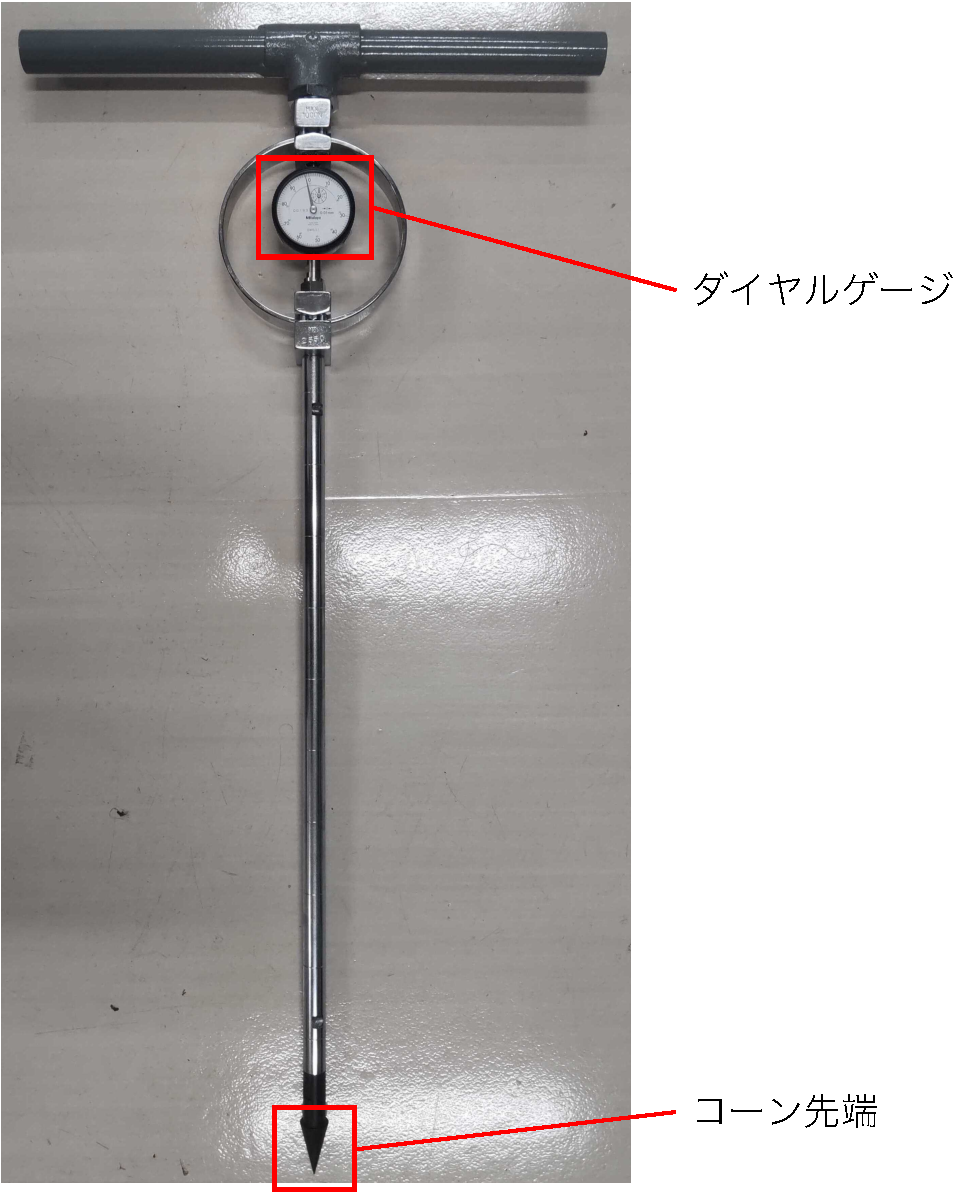
\includegraphics[keepaspectratio, width=0.5\linewidth]{cone_penetrometer.pdf}
  \caption{コーンペネトロメータ}
  \label{fig:cone_penetrometer}
\end{figure}

% textlint-disable
\vspace{3\zh}
\begin{table}[t]
  \caption{走行に必要なコーン指数(\protect\citeja{maff2015}を基に作成)}
  \label{tab:traffic_cone_index}
  \centering
  \begin{tabular}{cc}
    \toprule
    建設機械の種類                      & コーン指数[\si{\kN/\m^2}] \\
    \midrule
    超湿地ブルドーザー                    & 200以上                \\
    湿地ブルドーザー                     & 300以上                \\
    普通ブルドーザー(\SI{15}{\tonne}級程度) & 500以上                \\
    普通ブルドーザー(\SI{21}{\tonne}級程度) & 700以上                \\
    スクレープドーザ                     & 600以上                \\
                                 & (超湿地型は400以上)         \\
    被けん引式スクレーパ(小型)               & 700以上                \\
    自走式スクレーパ(小型)                 & 1,000以上              \\
    ダンプトラック                      & 1,200以上              \\
    \bottomrule
  \end{tabular}
\end{table}
% textlint-enable
\end{document}